\section{Modelling}
In order to achieve Model Predictive Control, it\textquotesingle s important to build a valid model of the dynamics of the RC car. In order to do so, it\textquotesingle  s important to understand the tire characteristics of this vehicle. This means there has to be a model for the tire characteristics as well. To build such a model, Data-Driven Model Design is used. 
To analyse the data of the test rig, a dynamical model is necessary. Accuracy of a dynamical model is closely related to the complexity of the model. However, due to the computational burden of these systems, a relative simple yet accurate model is necessary. Therefore, the Bicycle Model is chosen (Bron: 2014-01-0841 google drive pdf FIXME). With this model, it is possible to generate real time data that is still accurate. 

\begin{figure}
	\centering
		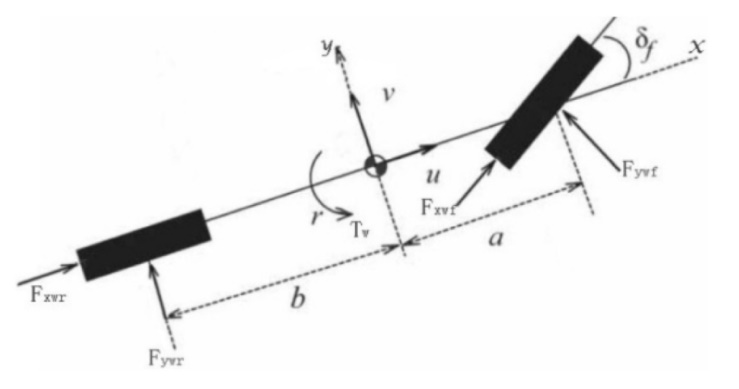
\includegraphics[scale=0.5]{figure/bicyclemodel.jpg}
	\label{fig:bicyclemodel}
	\caption{Bicycle model}
\end{figure}
Another suitable tire model would be the Dugoff tire model. This model provides a less accurate representation of the tire characteristics, but requires less variables. Even though fewer variables are needed though, more of the variables are unknown. Therefore, the Magic Formula model is easier to apply and gives a more accurate result, so to simplify calculations without a reduced quality of the final results, the Magic Formula model is chosen. 

\subsection{The Bicycle Model}
In the Bicycle Model, the car is represented as a rigid, two-dimensional, two-wheel vehicle with a xyz-coordinate system is fixed to the car frame. The front wheels are represented as one wheel and so are the rear wheels, as visible in figure \ref{fig:bicyclemodel}. This model comes with some important assumptions so there are some restrictions to test settings as well. The car should not move in the vertical (z-) position, nor rotate in the roll and pitch directions (around the x- and y- axes respectively). Therefore, movements are only possible in the x- and y-direction and as a rotation around the z-axis(yaw). 
	Furthermore, the bicycle model is divided in two parts: the linear and the nonlinear bicycle model. In general, a linear model is used for simplicity of the controller. Even though the performance of this model degrades at the limits of friction, it is demonstrated that using a linear tire model is still a good way of modelling (BRON: 2012-thesis-Kritayakirana GOOGLE DRIVE page 9). Even though, the non-linear bicycle model gives an even more accurate approximation of vehicle dynamics, and is therefore used.
	In the linear bicycle model, constant longitudinal velocity is assumed and lateral acceleration should not exceed 0.3 g . In order to meet these assumptions, the vehicle is not allowed to accelerate in the longitudinal direction while cornering. Therefore, data is not valid in the first seconds of each cornering test where the car has to accelerate. For the longitudinal motion tests however, it is necessary to accelerate and decelerate on the straight. If we still want to use the linear Bicycle Model for these experiments, the accelerations and decelerations cannot be very high. Otherwise this will result in inaccurate values given by this model.
	However, in some cases it will be helpful to use the nonlinear Bicycle Model. The limitations stated in the previous section will not occur. The nonlinear Bicycle Model will be used for tests where the longitudinal and lateral accelerations are high. This model comes with a larger set of equations and variables, and is solvable if the distribution of forces on the front and rear tires is known. In order to solve the equations, we assume a 50-50 distribution on these wheels, which makes sense if both the front and rear wheels are spinning at the same time. Because the wheels are connected to the same motor ,through differentials, and share the same properties, the forces acting on the wheels are approximately the same. 
	
\subsection{The Magic Formula}	
When the forces acting on the wheels of the car are known, thanks to the bicycle model values can be found to determine the slip angle \(\alpha\) and the slip ratio \(\kappa\). With these known, the tire characteristics can be determined using the Magic Formula tire model
 \ref{eq:magicformulaA}. 
\begin{equation}
	[F_{xwi} ,F_{ywi}] = MF(F_{zi},\alpha_{i},\kappa_{i},\mu) (i = f,r)
	\label{eq:magicformulaA} 
\end{equation}

In equation 1, the longitudinal force F_{x} and the lateral force F_{y} are calculated, using a the magic formula (MF) that depends on the gravitational force F_{z}, the slip angle \(\alpha\), the slip ratio \(\kappa\) and the friction coefficient \(\mu\). Except \(\mu\), all these variables are defined for two points on the bicycle model: the front wheel (f) and the rear wheel (r). 
	Equation \ref{eq:magicformulaA} can also be written as equation \ref{eq:magicformulaB}, which is stated by R.T. Uil of Eindhoven University. In this equation, variables B, C, D and E are introduced. B stands for the stiffness factor, C stands for the shape factor, D stands for the peak value and E stands for the curvature factor. This basic representation of the magic formula forms a graph that approximates the measured data and forms the tire characteristics of the vehicle. 

 \ref{eq:magicformulaB}. 
\begin{equation}
	R(\(\kappa\)) = D*sin{C*arctan[B*(1-E)*\(\kappa\)+E*arctan(B*\(\kappa\))]}
	\label{eq:magicformulaB} 
\end{equation}
